% Project 2 - EECS 499
% Author: Shaun Howard (smh150@case.edu)
\documentclass[conference]{IEEEtran} \usepackage[T1]{fontenc} \usepackage[backend=biber, style=ieee]{biblatex}
\addbibresource{report.bib} \usepackage[final]{microtype}

% graphics
\ifCLASSINFOpdf \usepackage[pdftex]{graphicx} % declare the path(s) where your graphic files are
  \graphicspath{{images/}} % and their extensions so you won't have to specify these with
  % every instance of \includegraphics
  \DeclareGraphicsExtensions{.jpeg,.png} \else
\fi

\usepackage{amsmath}
\usepackage[linesnumbered,ruled]{algorithm2e}
\usepackage{comment}
\usepackage[noend]{algpseudocode}

\newcommand{\sfunction}[1]{\textsf{\textsc{#1}}}
\algrenewcommand\algorithmicforall{\textbf{foreach}}
\algrenewcommand\algorithmicindent{.8em}

\begin{document}

\title{Turtlebot OMPL Motion Planner Benchmark}

\author{
 \IEEEauthorblockN{Shaun Howard}
 \IEEEauthorblockA{Electrical Engineering and Computer Science Department\\
                   Case Western Reserve University\\ 
                   Cleveland, Ohio 44106\\
                   Email: smh150@case.edu}
}

% make the title area
\maketitle

% As a general rule, do not put math, special symbols or citations
% in the abstract
\begin{abstract}
Motion planning is an important part of modern robotics. Motion plans are intricate and sometimes time-consuming to develop in real scenarios.
The modern abstraction of motion planning has left most researchers to focus on new things. However, sometimes we take for granted the solutions
we are given to problems that we encounter everyday. Although the solution we interpret as right might approximately solve the problem, it may not 
be the best solution available. This paper focuses on analysing the pros and cons of all the modern geometric planners OMPL has to offer in order to
determine the best choice where obstacle avoidance and complex path planning are necessary. We also explore their statistical similarities and differences using the OMPL 
Benchmark libraries. 
The goal of this paper is to determine if the planners we currently use in the robotics industry will be the best and most efficient choices for the 
tasks of tomorrow.
\end{abstract}

\section{Introduction} \label{Introduction}

The search for accurate and quick planning algorithms has grown in recent years with major breakthroughs in memory architecture, processing unit speed and 
parallel processing. Robots inherently have higher degrees of freedom and more dimensions of parameters to tweak in their environments. Several planning methods exist that 
intricately check environment surroundings, configuration space and workspace constraints, and validate
that solutions can be executed by the robot due to differential or joint limits and constraints. Current planners may or may not be able to cope with dynamic environment 
updates that are not predictable by some sort of probabilistic approach. Spontaneity in determining solutions within a small window of time is a valuable trait of a 
modern motion planner. Obstacles may have complex behaviours that many robots may not understand quick enough to react. Today, with autonomous vehicles on the rise, 
quicker and more accurate planners are needed to support continuous and dynamic behaviour.

Sampling-based motion planning techniques were developed to facilitate the search for new solutions in less time. These planners were developed to randomly explore the
high-dimensional search space of modern robots in order to spontaneously find unique solutions to problems. The idea of these planners is to randomly generate a graph
of possible nodes to explore for the robot, represented typically within a bounded workspace, and connect them from either direction, if possible, to reach the goal 
without collisions from start to finish. Sometimes, solutions are picked that meet the constraints of the given task being executed for some probability of the time, 
while the remainder of the time, the planner approaches the goal. Some planners can solve many problem queries from one graph. A primary single-query sampling-based approach to 
motion planning is the Rapidly-exploring Random Tree (RRT). The RRT is useful for solving one-off problems quickly in a random, forward-thinking behavior.  The RRT solutions are
not reproducible, which can cause performance headaches at times when plans are not easy but are redundant. A primary multi-query sampling-based technique, used especially for 
redundant situations like driving, is the probabilistic roadmap (PRM). This planner, which saves a mapping of the environment based on the PRM construction algorithm outlined in
a section to come. Improvements have been made to both planning algorithms to allow for quicker and more compact motion plans such as the RRT*, LazyRRT, LazyPRM. Alternative
algorithms that combine the renditions of the RRT, PRM or another main technique combined with local planners have been created such as the Fast Marching Tree 
Star (FMT*), SPARS, SPARS2, PDST, and STRIDE. Many of these alternatives may perform faster than their RRT and PRM counterparts. The true goal of  this paper will be
to determine if any of these alternative planners will better serve as the go-to planner of tomorrow for high-dimensional problems than the widely accepted RRT or PRM extensions.

A straightforward way to test the performance of these algorithms is to implement an instance 
of the Open Motion Planning Library (OMPL), as described by Șucan, Moll, and Kavraki in \cite{ompl}. The OMPL has several implementations of motion planning algorithms 
including those mentioned above. The OMPL Benchmark library, as presented in \cite{ompl_benchmark}, will be useful for benchmarking those algorithms and acquiring the
data necessary for benchmark comparison. The benchmark library will run each algorithm on each of the problem descriptions from start to goal locations. 
Experiments can thus be chained together to tremendously speed up benchmarking.

The turtlebot simulator is an appropriate simulator model for OMPL benchmarking purposes. A two-dimensional costmap of the environment surroundings of the Turtlebot
will be utilized as provided by ROS and Clearpath Robotics in the occupancy\_grid\_utils and costmap\_2d software libraries. The turtlebot simulator environment and costmap 
are displayed in figure 1. Autonomous driving requires accurate and efficient motion planning. Given the simplicity of the OMPL planner interface, the outcomes of the benchmark
for OMPL algorithms will be highly generalizable for application to modern mobile robotics. that is common and easy to set-up for modern. It will also be appropriate to constraint motion plans based on differential constraints of the turtlebot, as most vehicles similarly have. Overall, the 
AMCL planner with a generated map of a test turtlebot environment will be used for robot localization benchmarking purposes. The map will be represented to the robot by 
means of a 2-dimensional costmap, generated primarily by the dynamic window approach (DWA) planner provided by ROS. The DWA implemented by ROS is based on the 
methodology proposed by D. Fox, W. Burgard, and S. Thrun. in \cite{dwa}. The benchmarking planner will inherit properties from the BaseGlobalPlanner provided by ROS in 
order to act as a true motion planning plug-in for compatibility with components of the ROS motion planning framework like the Rviz robot interaction and visualization 
application.

The next sections describe background information for the problem domain, the algorithms available via OMPL for the planning tasks, their pros and cons, their benchmark 
test experiments, results and comparison between the algorithms using OMPL benchmark planner statistics.

\section{Background Information} \label{Background Information}

Several aspects of the planners will be evaluated in the benchmarks of this paper. The concepts spanned will include the properties of asymptotic optimality, probabilistic 
completeness and computation complexity. Each of these properties for the planners that will be benchmarked in this paper will affects its overall performance against
the other algorithms. Each of these factors holistically affect planning time, simplification time, solution length, and the number of iterations
taken by each algorithm to find the best cost path it can. The definitions for each of these algorithms will be discussed next.

\subsection{Probabilistic Completeness} \label{Probabilistic Completeness}

\subsection{Asymptotic Optimality} \label{Asymptotic Optimality}

\subsection{Computational Complexity} \label{Computational Complexity}

\section{Planning Algorithms} \label{Planning Algorithms}

\subsection{Rapidly-Exploring Random Tree} \label{RRT}
The rapidly-exploring random tree algorithm was pioneered by S. LaValle and J. Kuffner around 2000. The RRT was designed to rapidly and randomly explore high-dimensional
state space in a completely configurable but always sampling-based method. They proved that it is probabilistically complete when they implemented it in their 2001 paper 
\cite{random_kinodynamics}, where they experiment with an under-actuated spacecraft that performs complex maneuvers amongst other robots and compare the performance 
results. The pseudocode for the algorithm is displayed in figure 2.

\begin{figure}
\label{figure2} 
\centering 
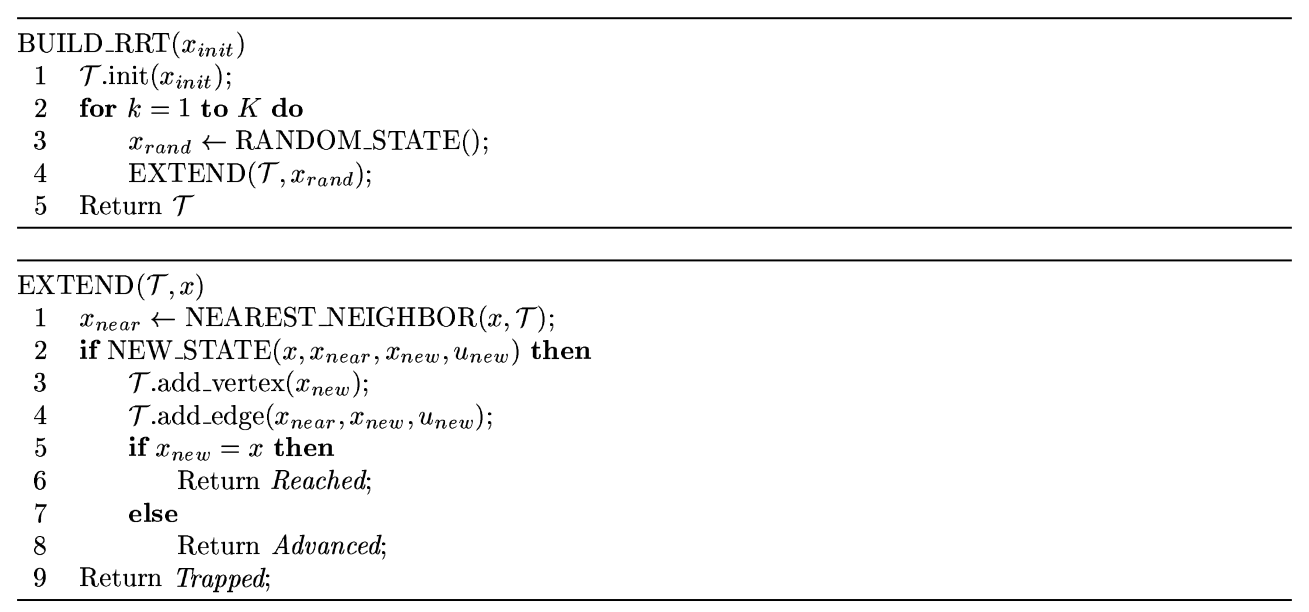
\includegraphics[width=0.49\textwidth]{rrt}
\caption{RRT pseudocode}
\end{figure}

The upsides to the RRT planner are the following:
\begin{itemize}
\item probabilistically complete
\item performance
\item no preprocessing
\item simplification of higher dimensionality
\item good with differential constraints
\item good with non-linear systems
\end{itemize}

The downsides of the RRT planner are the following:
\begin{itemize}
\item no memory for multiple queries
\item optimality is not guaranteed
\end{itemize}

\subsection{RRT*} \label{RRT*}
The heuristically-driven RRT, RRT*, is a rendition of the RRT that uses a distance or obstacle-based cost heuristic to reach the goal. The RRT* is approximately 
asymptotically optimal, like the well-known A* algorithm. This version of the RRT planning algorithm was introduced in \cite{sampling_star}. Since the RRT* is almost
optimal, this means that the cost of the returned solution path converges almost definitely to the optimal solution for that planning problem. The pseudocode for the
RRT* algorithm is in figure 3.

\begin{figure}
\label{figure3} 
\centering 
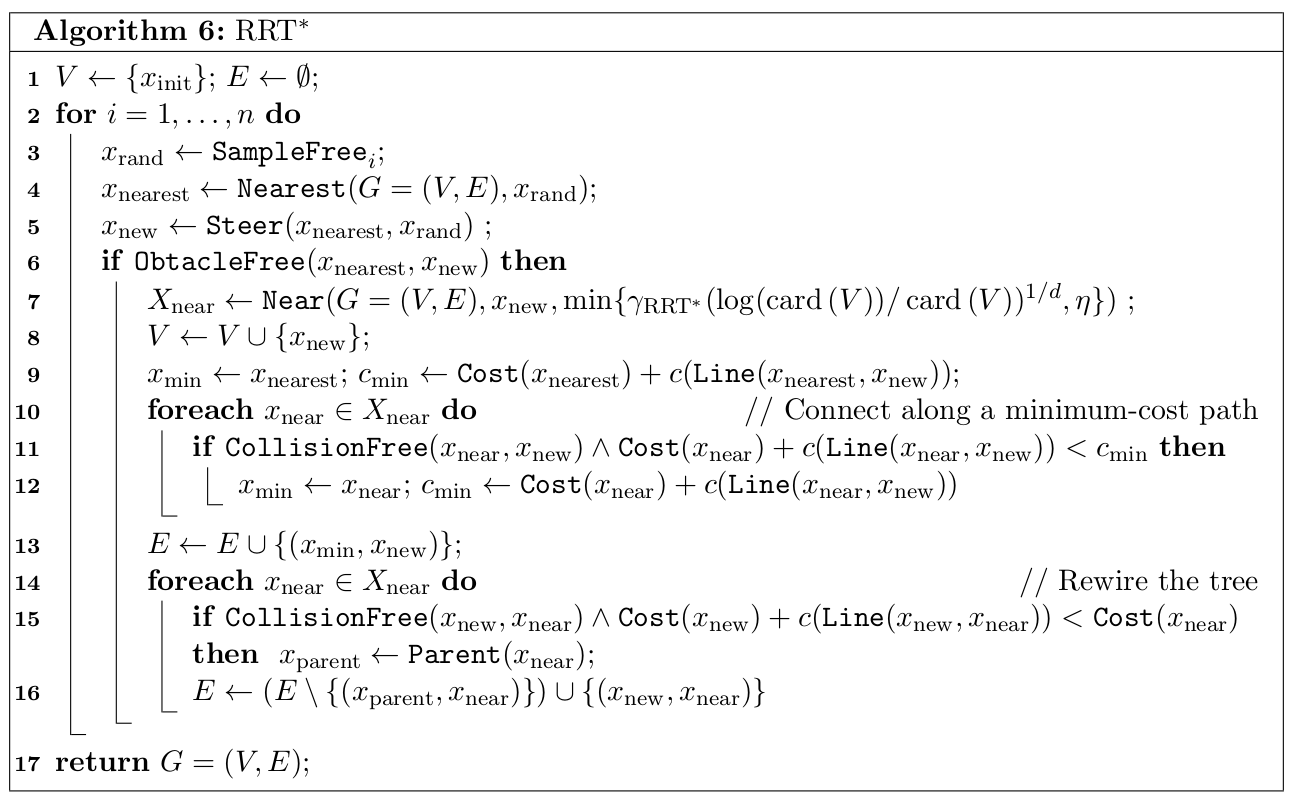
\includegraphics[width=0.49\textwidth]{rrt_star}
\caption{RRT* pseudocode}
\end{figure}

The pros of the RRT* algorithm follow:
\begin{itemize}
\item probabilistically complete
\item asymptotically optimal
\item monotone convergence
\end{itemize}

The cons of the RRT* algorithm follow:
\begin{itemize}
\item cons of RRT, such as no memory for solutions
\end{itemize}


\subsection{LazyRRT} \label{LazyRRT}
The lazy RRT is a rendition of the RRT that explores only part of the random tree that is necessary to solve the current query. It was first introduced by R. Bohlin and 
L. Kavraki in \cite{lazy_rrt}. The lazy RRT is an RRT optimized for single-query, high-dimensional, uncluttered, global configuration spaces. The lazy RRT aims to 
minimize the number of collision checks performed during the RRT planning process. This addition to the RRT makes for a more efficient implementation of the RRT that has 
a better runtime in the general case. Pseudocode for the LazyRRT is omitted for brevity purposes. The C++ namespace reference in OMPL is ompl::geometric::LazyRRT for
the algorithm implementation application programming interface (API).

The good features of the LazyRRT are:
\begin{itemize}
\item speedup from reduced collision checking
\item same as RRT
\end{itemize}

The bad features of the LazyRRT are:
\begin{itemize}
\item cons of RRT minus collision-checking inefficiencies
\item worst case runtime matches RRT worst case runtime due to frequent collision checks
\end{itemize}

\subsection{Probabilistic Roadmap} \label{PRM}
The probabilistic roadmap was first released the to the public in 1996 with \cite{prm}. The goal was to build a map of possible nodes to visit amongst the obstacles in 
the environment. The algorithm is based on a static map of the robot's environment. The planner has two phases: a learning and a query phase. The nodes represent 
collision-free robot configurations, while the edges represent clear paths to travel between those nodes. The PRM is known to excel with the help of a local planner like 
the ROS DWA planner that will be used in this benchmark. The construction algorithm pseudocode is presented in figure 4.

\begin{figure}
\label{figure4} 
\centering 
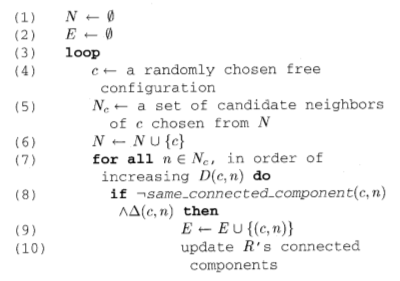
\includegraphics[width=0.49\textwidth]{prm}
\caption{PRM construction phase pseudocode}
\end{figure}

The pros of the PRM:
\begin{itemize}
\item probabilistically complete
\item monotone convergence
\end{itemize}

The cons of the PRM:
\begin{itemize}
\item issues handling differential constraints
\item not guaranteed to be asymptotically optimal
\item slower query time that RRT
\item inability to deal with environment changes without reconstruction
\end{itemize}

\subsection{LazyPRM} \label{LazyPRM}
The lazy PRM is an enhanced version of the PRM that lazily checks for collisions. The lazy PRM was described as an enhancement to the PRM in \cite{lazy_prm}. Initially, 
the planner assumes that all randomly-generated configurations are collision-free. Once nodes or edges with collisions are found, they are removed from the roadmap and
new nodes and/or edges are generated and inserted. This process is repeated until a collision-free solution is found. The theme of the planner is to minimize the number
of collision checks needed to reach a goal. The high-level overview of the LazyPRM is shown in figure 5.

\begin{figure}
\label{figure5} 
\centering 
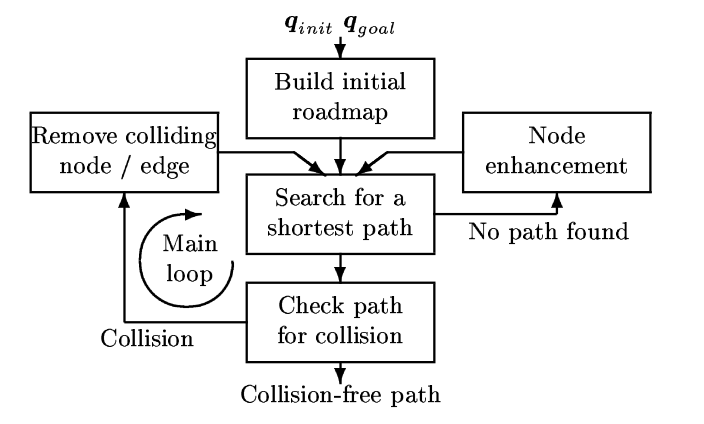
\includegraphics[width=0.49\textwidth]{lazy_prm}
\caption{LazyPRM overview}
\end{figure}

The pros of the LazyPRM:
\begin{itemize}
\item pros of PRM
\item speedup from infrequent collision checking
\end{itemize}

The cons of the LazyPRM:
\begin{itemize}
\item cons of PRM minus collision checking inefficiencies
\item worst case runtime matches PRM worst case runtime due to frequent collision checks
\end{itemize}

\subsection{SPArse Roadmap Spanner Algorithm} \label{SPARS}
The SPARS planner is a divergence from the typical sampling-based PRM and heuristically-driven PRM star algorithms. The work in \cite{spars} develops a method of planning 
that shows finite-size data structures can have close to optimal properties without spanning over as much space as previously integrated PRM* graph spanners. Query
resolution for the SPARS planner is faster than for mainstream PRM*-based planners. Although most PRM algorithms require the map to grow infinitely large to converge to 
the desired state of optimality, the SPARS algorithm satisfies near-optimality, workspace bounds and completeness criteria to generate solutions much faster than typical
PRM planners, while benefiting from the same upsides of the PRM approaches. After smoothing, paths are found to be much shorter than paths developed by other algorithms.

The SPARS planner provides probabilistic completeness and near asymptotic optimality by building two graphs in parallel. The first graph is a dense asymptotically-optimal
PRM*-based roadmap and the second graphs is the spanner of the first graph. The SPARS pseudocode can be found in figure 6.

\begin{figure}
\label{figure6} 
\centering 
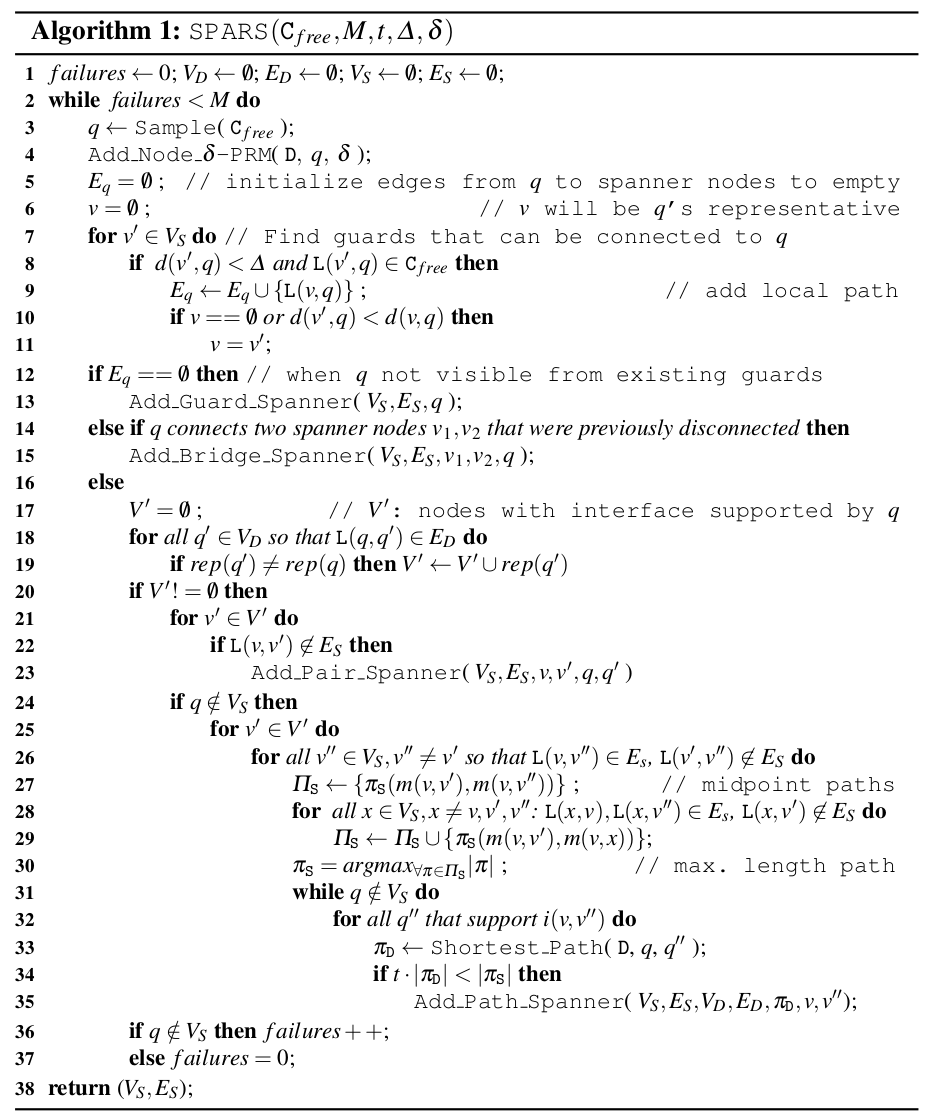
\includegraphics[width=0.49\textwidth]{spars}
\caption{SPARS pseudocode}
\end{figure}

The pros of the SPARS planner:
\begin{itemize}
 \item highly efficient
 \item highly generalizable
 \item small solution plans
 \item probabilistically complete
 \item optimal solutions
 \item does not grow out of memory like other methods
\end{itemize}

The cons of the SPARS planner:
\begin{itemize}
 \item maintains two graphs to meet completeness and optimality criteria
 \item inefficiencies fixed in SPARS2 planner
\end{itemize}

\subsection{SPArse Roadmap Spanner Algorithm Two} \label{SPARS2}
The SPARS2 planner was introduced as a simplification of the SPARS algorithm in \cite{spars_two}. As the SPARS planner uses two graphs to meet probabilistic 
completeness and near-optimality criteria, the SPARS2 planner reveals it is possible to relax the sampling conditions without using a dense graph. Desirable properties
of the SPARS algorithm are maintained in SPARS2, such as the decrease in probability to zero of adding new nodes to the roadmap over time. The SPARS2 algorithm
generates graphs that are orders of magnitude smaller than the PRM*-based solutions. Hence, the SPARS2 algorithm is competitively performant between the other sampling-
based approaches to path planning. The SPARS2 pseudocode can be found in figure 7.

\begin{figure}
\label{figure7} 
\centering 
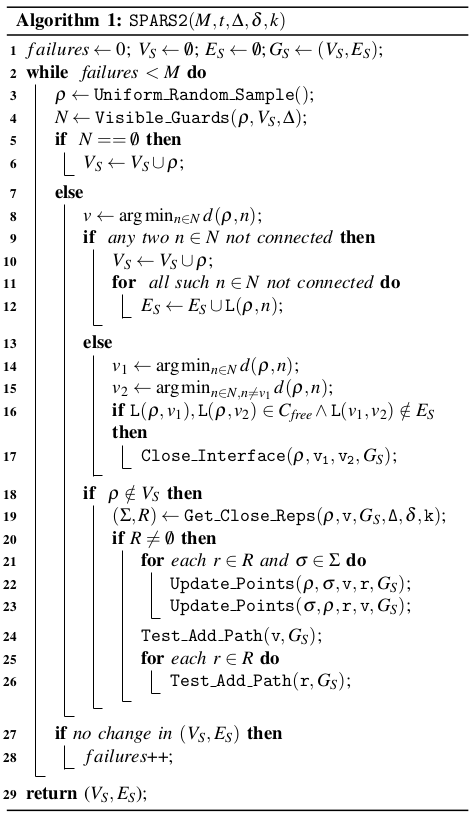
\includegraphics[width=0.49\textwidth]{spars2}
\caption{SPARS2 pseudocode}
\end{figure}

The upsides of the SPARS2 planner:
\begin{itemize}
 \item pros of SPARS
 \item small growth rate and solution size, even less than SPARS
\end{itemize}

The downsides of the SPARS2 planner:
\begin{itemize}
 \item compromise in final spanner size as compared to SPARS spanner
\end{itemize}

\subsection{Path-Directed Subdivision Trees} \label{PDST}
The PDST planner was designed specifically for systems with inherent drift, under-actuation and discrete changes. The approach utilizes a sampling-based
approach and path-directed subdivision to solve complex planning problems. The approach was proposed and applied in \cite{pdst} to the game Koules, which exhibits 
dynamical characteristics of complex motion planning problems. The algorithm was applied to scenarios with up to 85 dimensions, but obviously suffered from
memory overhead issues. Hence, the PDST is slower as memory size grows due to usage of hard disk page file and other hardware limitations, but the algorithm
should be applicable to a lower dimensional motion planning problem as for the turtlebot benchmark scenarios in this paper. The pseudocode for the algorithm is displayed in figure 8.

\begin{figure}
\label{figure8} 
\centering 
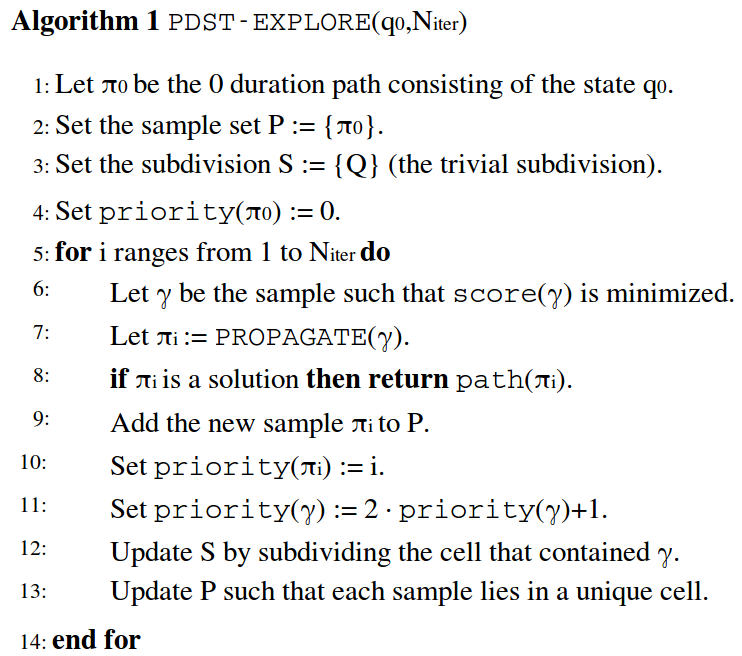
\includegraphics[width=0.49\textwidth]{pdst}
\caption{PDST pseudocode}
\end{figure}

Good features of the PDST algorithm follow:
\begin{itemize}
 \item good for severe under-actuation
 \item good for significant drift
 \item good for high dimensionality
 \item appropriate for discrete system changes that occur at boundary conditions
 \item applicable to systems which are not reducible to a system with lower order dynamics
\end{itemize}

Bad features of the PDST algorithm follow:
\begin{itemize}
 \item high state complexity
 \item requires path sampling representation for efficiency sake
 \item once the number of states needed to represent the search tree exceeds the size of the virtual memory, the speed decreases significantly due to disk accesses
\end{itemize}

\subsection{Fast Marching Tree Star} \label{FMT*}
The FMT* algorithm is a sampling-based planning algorithm that is targeted to solve complex motion planning problems in high-dimensional configuration space. The
algorithm is shown to be faster than both of its RRT* and the PRM* rivals. Unlike the other planners, the FMT* utilizes a lazy and recursive dynamic programming 
strategy to grow a tree of paths from a preselected number of probabilistically-drawn sample nodes. By doing this, it combines the features of both single and multi-
query path planners. It is influenced by the Fast Marching Method for solving Eikonal equations. It is described in \cite{fmt_star} and analyzed under the
notion of probability of convergence rather than analysis of sure converge like other planners. The convergence rate is bounded in big-O time and the algorithm
is found to be asymptotically-optimal even with various factors such as non-uniformly sampled nodes. The algorithm is found to generate much better solutions
that its RRT and PRM counterparts mostly in higher-dimensional configuration spaces or where collision-checking is inefficient. In figure 9 is the FMT* pseudocode.

\begin{figure}
\label{figure9} 
\centering 
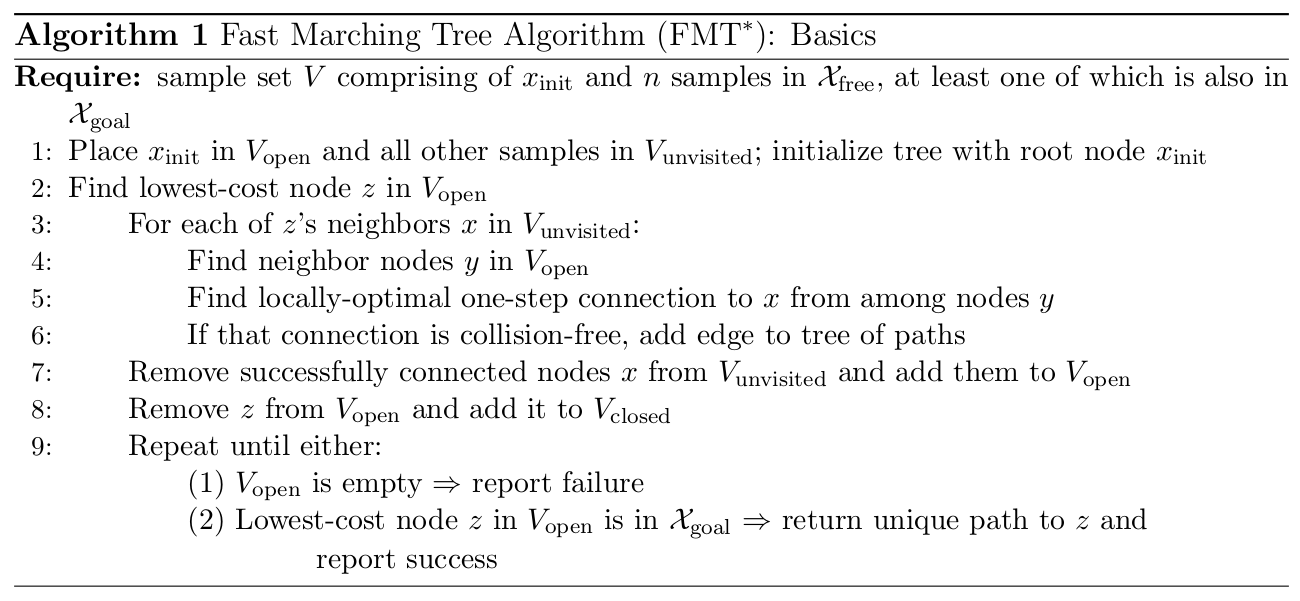
\includegraphics[width=0.49\textwidth]{fmt_star}
\caption{FMT* pseudocode}
\end{figure}

The beneficial aspects of the FMT* algorithm are the following:
\begin{itemize}
 \item faster than the PRM*
 \item builds paths in a tree-like structure rather than a graph like PRM
 \item satisfies differential constraints in a forward fashion unlike graph-based algorithms (PRM)
 \item higher quality and more consistent solutions than RRT* given the uniformly larger error bars on the RRT* versus FMT* solution
 \item optimal without obstacles
\end{itemize}

The detrimental aspects of the FMT* algorithm are the following:
\begin{itemize}
 \item only nearly optimal with obstacles
\end{itemize}

\subsection{Search Tree with Resolution Independent Density Estimation} \label{STRIDE}
The STRIDE algorithm was designed to support rapidly-exploring path planning in high-dimensional space with over 10 dimensions. The algorithm was first introduced
in \cite{stride}. The algorithm is mostly parameter-free due to the utilization of a Geometric Near-neighbor access tree (GNAT) to estimate the sampling density of the 
configuration space. This results in an implicitly resolution-independent Voronoi partitioning scheme to provide sampling density estimates, guiding the planner 
naturally to unexplored regions of configuration space. STRIDE is also capable of exploring the full dimensionality of the search space given that GNAT only requires a 
valid distance metric. Results in \cite{stride} show that the algorithm performs much better than others like the RRT and PRM when the search space is defined
by narrow passageways. Thus, the algorithm seems an appropriate match for a motion planning problem where tight passageways are common as in autonomous navigation.
Pseudocode for the algorithm is displayed in figure 10.

\begin{figure}
\label{figure10} 
\centering 
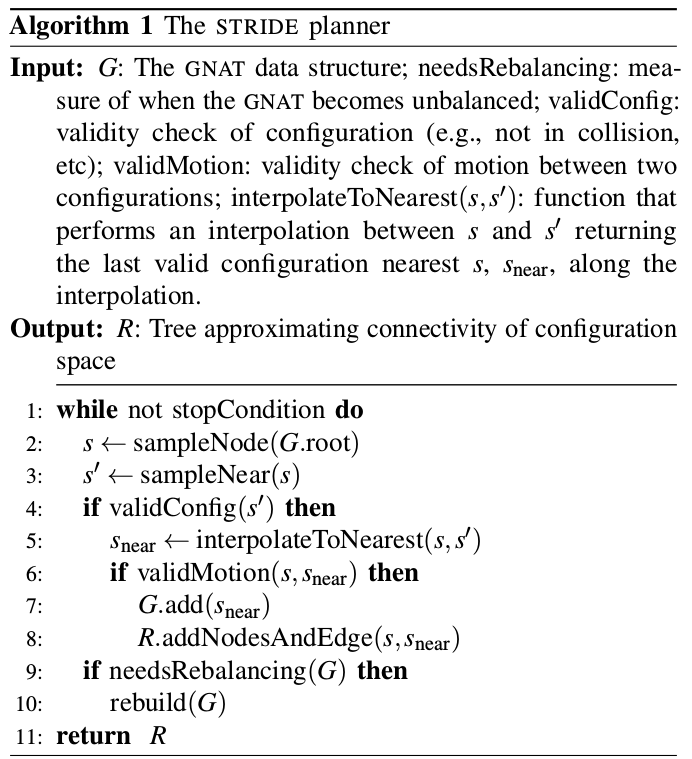
\includegraphics[width=0.49\textwidth]{stride}
\caption{STRIDE pseudocode}
\end{figure}

The best features of the STRIDE algorithm are:
\begin{itemize}
 \item Voronoi partitioning scheme
 \item resolution independent
 \item rapid exploration of unexplored regions
 \item performance improvements over other similar planners
 \item uses a data structure that enables it to produce density estimates fully in configuration space
 \item much more efficient than other planners
 \item smaller solution paths
 \item shorter runtime
\end{itemize}

The worst features of the STRIDE algorithm are:
\begin{itemize}
 \item not guaranteed optimal
 \item not guaranteed probabilistically complete
\end{itemize}

\section{Benchmark Scenarios} \label{Benchmark Scenarios}

Three benchmark scenarios will be examined between all of the algorithms. Given the differing structures between some of the algorithms, they do not all
have consistent data collection from the OMPL Benchmark library, but many of them align on given output information about the algorithm useful for benchmarking
and comparison. From the acquired data, we will then determine the best choice algorithm for each planning scenario. The first scenario will be when there is clearly a 
collision-free path from start to finish along the map. The second scenario will include a sparse area of objects that obscure the vision between the turtlebot and 
the goal but are not too confusing for the path planner. The third scenario will consist of a path through several objects in a dense mapping of objects along the map. 
The goal will not directly be visible from the turtlebot starting location, nor will it be too easy to find without utilizing the environment cost map.

For each of the benchmark scenarios, rules will be set across the board. Each planner will be run 5 times with 500 megabytes maximum memory. Each planner will be allowed 5 
seconds per run before being terminated. The planners will not be operated in a multi-threaded fashion. The planners will each be run with their default parameters. Some 
planners will be able to produce approximate solutions and/or optimize solutions while others will not based on OMPL implementation. Solutions will be simplified using OMPL 
Simple Setup procedures, and the time to simplify each planner's path will be recorded. The workspace will be bounded by the environment map in all benchmarks. The planners 
will be optimized to seek short path length. The benchmark scenarios and results follow.

\subsection{Obstacle-Free Path} \label{Obstacle-free Path}

The obstacle-free portion of the map utilized for the first benchmarking scenario is show in figure 11. This scenario is useful for determining which planner is the
best for clear path planning without obscurities.

\begin{figure}
\label{figure11} 
\centering 
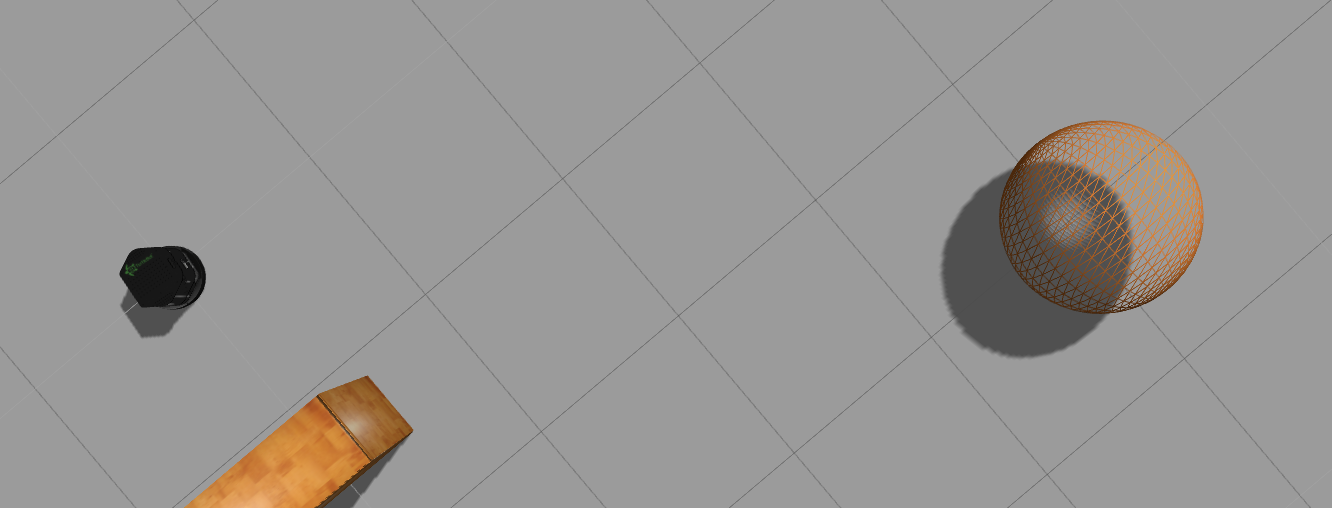
\includegraphics[width=0.49\textwidth]{scenario_1}
\caption{Obstacle-free path-planning scenario}
\end{figure}

\begin{figure}
\label{figure12} 
\centering 
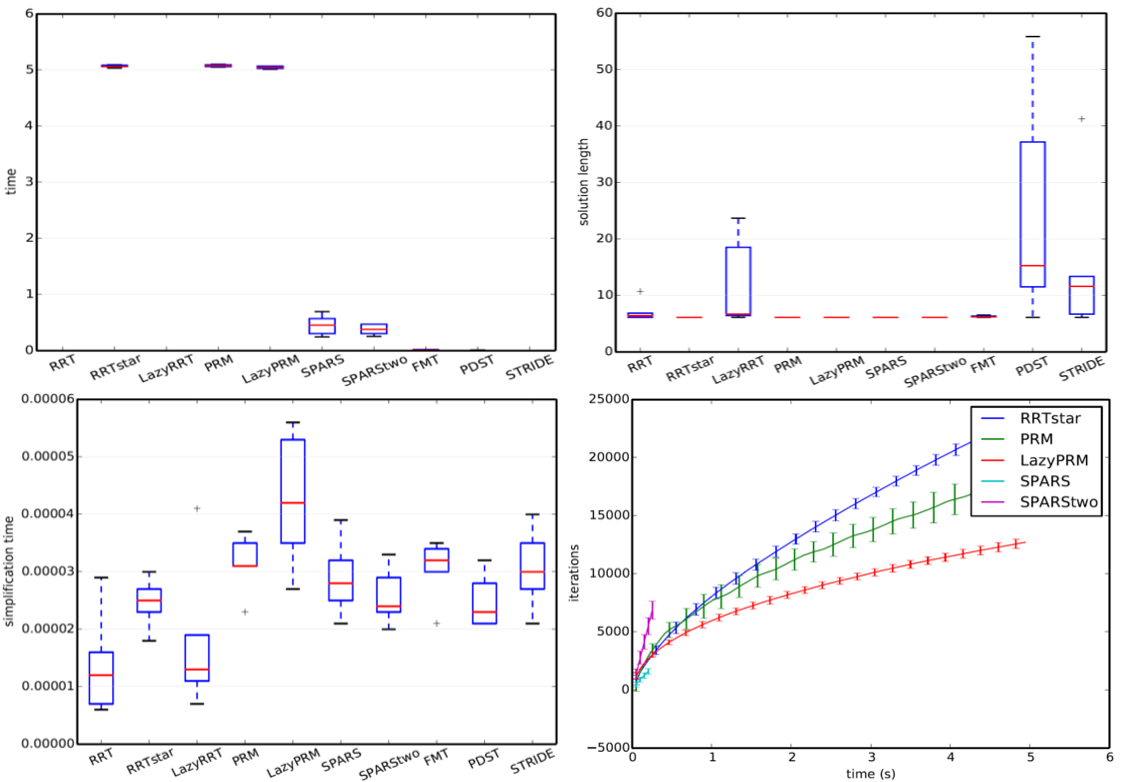
\includegraphics[width=0.49\textwidth]{s1_outcomes}
\caption{Obstacle-free scenario outcomes}
\end{figure}

The important graphs of algorithms produced during this run are tiled in figure 12. From the results we reflect that all planners were able to find an exact solution
for this planning problem. The planners in order from minimum to maximum amount of time were the following: STRIDE, PDST, FMT*, SPARS2, SPARS, LazyPRM, PRM and RRT*. 
Surprisingly, the planner that took the least amount of time to determine the exact solution was the STRIDE planner at approximately 0 seconds on average. The number
of iterations taken by each planner, though, showed a slightly different trend. In terms of iterations, the order from least to greatest follows: SPARS, SPARS2, LazyPRM, PRM,
and RRT*. The SPARS planner took approximately 3000 iterations to converge on average. It happened to perform orders of magnitude faster than the RRT* and PRM-based planners, which 
each took at least 12,500 iterations to converge on average. The SPARS2 planner took about 8,000 more iterations to converge than the SPARS planner at 11,000 iterations on average.
The FMT*, PDST, and STRIDE methods were omitted from this benchmark.

The solution length statistics show that many of the planners found the shortest path for the planning problem. These all-star planners for scenario 1 are the following: RRT*,
PRM, LazyPRM, SPARS, and SPARS2. The other planners had close path distances on average, but some planners like the LazyRRT, PDST and STRIDE had a high amount of variance in 
their solution length values. The FMT* planner was an exceptional case, as it consistently had a slightly higher solution length average than the shortest path.

Continuing, we observe that the amount of time taken by the path simplification algorithm to simplify the generated paths did not correlate with the time necessary to determine
the solutions. Although planners found the exact solution to the problem, those solutions varied in segment count and solution smoothness. The planners based on the RRT
and PRM varied in all elements of the benchmark. Those algorithms were neck in neck for advantages and disadvantages, but the lazy collision-checking versions tended to dominate. 
The PDST and STRIDE algorithms tended to produce longer paths than the other algorithms. However, the smoothness of some these paths was much higher than that of the other 
planners, despite the length, and the simplification time shows how far from simplified those solutions actually were via runtime chart. Despite the differences, all generated 
solutions were able to be simplified and some of the generated paths were already simplified, thus not needing simplification. The simplification time in order from least to greatest was as follows: RRT, LazyRRT, RRT*, PDST, SPARS2, SPARS, STRIDE, PRM, FMT*, and lastly, the LazyPRM. 

Analysing the statistical graphs produced by the OMPL benchmark, we can determine which planners were the quickest, which planners had the shortest solutions, which planners
were more performance efficient, which planners had the smoothest solutions and which planners consumed the most memory.

In terms of time, the quickest planners were the STRIDE, PDST, FMT*, SPARS2, and SPARS planners. These all had the best times of the bunch, taking less than 1 second to solve.
In terms of solution length, the planners with the shortest solutions were all but the LazyRRT and PDST algorithms, which had high amounts of variation in output. In terms of
performance efficiency, the planners that were best off were the SPARS, SPARS2, and LazyPRM planners. Surely, the STRIDE and FMT* planners were also neck in neck, but they were
omitted from this benchmark. In terms of solution smoothness, the top algorithms were the LazyRRT, STRIDE, and PDST. Many algorithms were omitted from that benchmark,
so nothing can be said about their smoothness. Lastly, in terms of minimal memory consumption, the top contenders were the RRT and PRM algorithms. All other algorithms 
consumed much more memory than these, mostly due to difference in planning approach. The SPARS and SPARS2 algorithms both consumed less than all other remaining planners, which
include PDST and STRIDE, which consumed the most memory.

From these results, we can conclude that the best planners for an obstacle-free environment are either of the SPARS or SPARS2 planners.

\subsection{Sparse Obstacle Map} \label{Sparse Obstacle Map}

The sparse obstacle portion of the map utilized for the second benchmarking scenario is displayed in figure 13. This scenario is useful for determining which planner is 
the best choice for path planning with sparsely laid obscurities in the path from start to goal. The planner will start from a location of the turtlebot that cannot see
the goal. The environment between the turtlebot and the goal will be straightforward to draw a path from a top-down 2-D view.

\begin{figure}
\label{figure13} 
\centering 
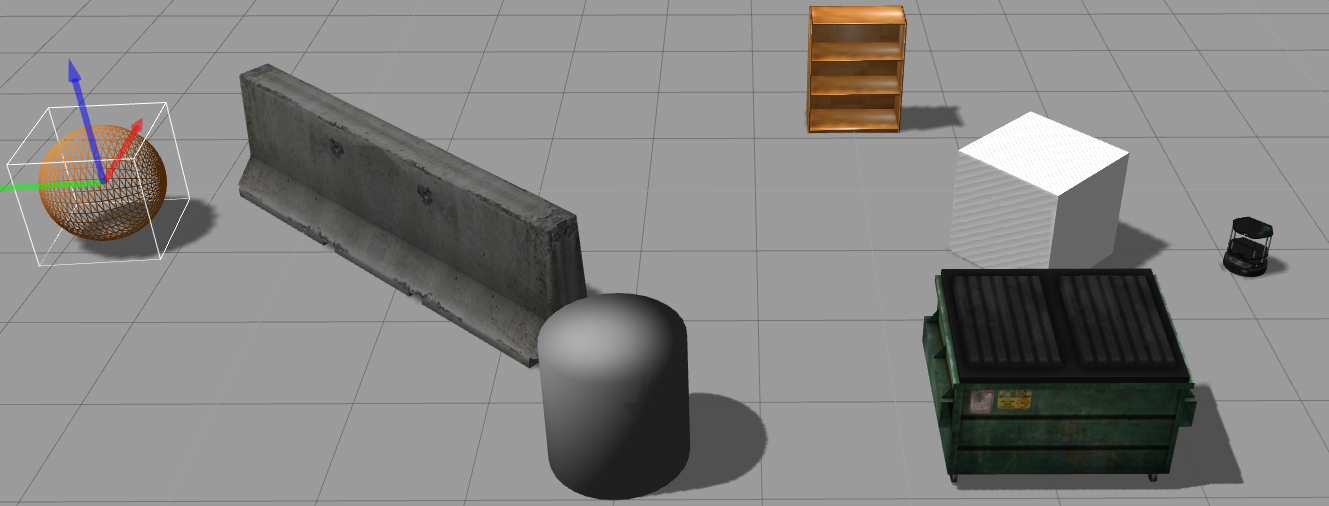
\includegraphics[width=0.49\textwidth]{scenario_2}
\caption{Sparse obstacle path-planning scenario}
\end{figure}

\begin{figure}
\label{figure14} 
\centering 
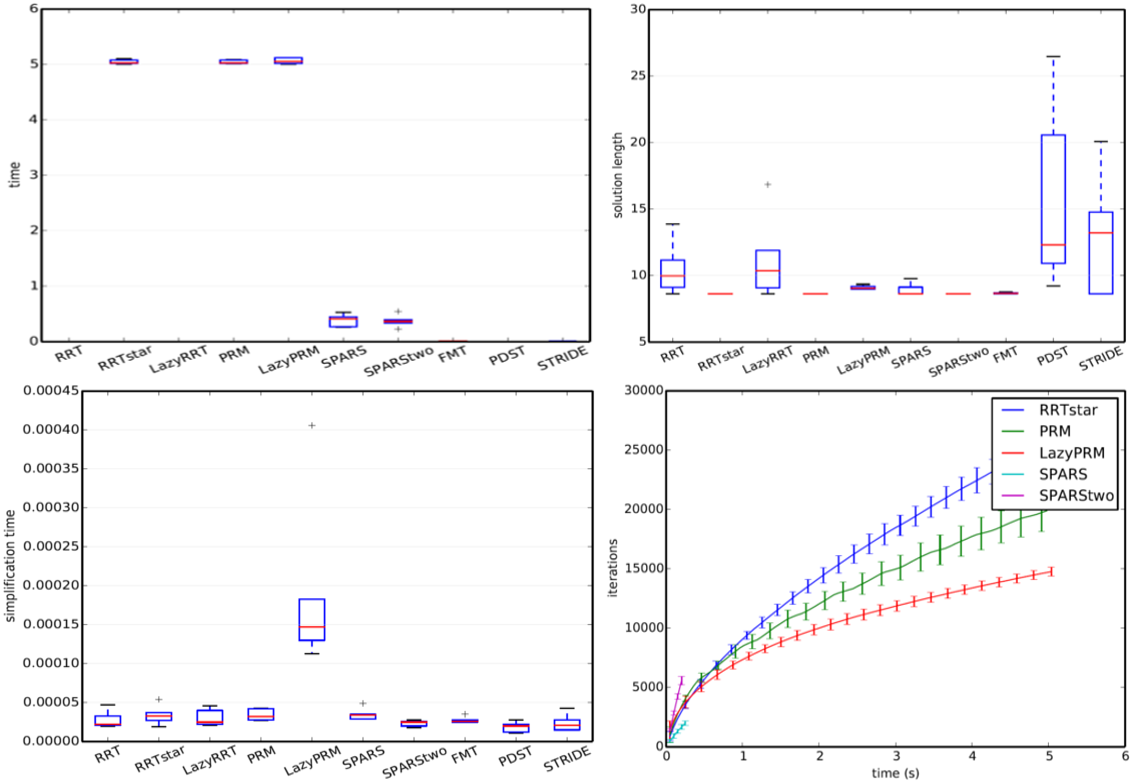
\includegraphics[width=0.49\textwidth]{s2_outcomes}
\caption{Sparse obstacle scenario outcomes}
\end{figure}

The important graphs of algorithms produced during this run are tiled in figure 14. From the results we reflect that all planners were able to find an exact solution
for this planning problem. The planners in order from minimum to maximum amount of time were the following: PDST, STRIDE, FMT*, SPARS2, SPARS, PRM, RRT*, and LazyPRM. 
Surprisingly, the planner that took the least amount of time to determine the exact solution was the PDST planner at approximately 0 seconds on average. The number
of iterations taken by each planner, again, showed a slightly different trend. In terms of iterations, the order from least to greatest follows: SPARS, SPARS2, LazyPRM, PRM,
and RRT*. The SPARS planner took approximately 3000 iterations to converge on average as before. It happened to perform orders of magnitude faster than the RRT* and PRM-based 
planners, which each took at least 14,500 iterations to converge on average. The SPARS2 planner took about 7,000 more iterations to converge than the SPARS planner at 10,500 
iterations on average. The FMT*, PDST, and STRIDE methods were again omitted from this benchmark.

The solution length statistics continued to show that many of the planners found the shortest path for the planning problem. The shortest path planners for scenario 2 were not the 
same as those for scenario 1 and are in this order: RRT*, PRM, SPARS, SPARS2 and FMT*. The LazyPRM was also close in having the shortest path found. The other planners, however,
had large amounts of variance in their solutions, showing that they are not consistent in generating solutions.

Carrying on, we observe that the amount of time taken by the path simplification algorithm was consistent across the board except for the Lazy PRM, whihc took 1.5 thousands of a
second on average. The simplification time in order from least to greatest was as follows: PDST, STRIDE, RRT, SPARS2, FMT*, LazyRRT, PRM, RRT*, SPARS, and lastly, the LazyPRM. As
revealed by scenario 1, the LazyPRM tends to take the greatest amount of time to simplify of all the algorithms. This reveals that the LazyPRM produces paths with more segments
than the other planners, which is upheld by the benchmark results. The LazyPRM tended to have 5 solution segments on average, more than all the other planners. Despite these
differences, the LazyPRM planner upheld a substantial rivalry to the other planners.

In terms of time, the quickest planners were again the STRIDE, PDST, FMT*, SPARS2, and SPARS planners. These all took less than 1 second to solve.
In terms of solution length, the planners with the shortest solutions were the RRT*, PRM, SPARS2, FMT* and SPARS planners. The other planners had high amounts of variation in 
output. In terms of performance efficiency, the planners that were best off were the SPARS, SPARS2, and LazyPRM planners. In terms of solution smoothness, the worst algorithms
were the RRT, STRIDE, and LazyPRM, in ascending order. The algorithms with smoothest solutions were SPARS, LazyRRT and PDST. Lastly, in terms of minimal memory consumption, the top 
contenders were the RRT* and LazyRRT algorithms, due to their single query planning behaviour. These algorithms consumed much less memory than all the other algorithms, which
were all equivalent in memory consumption during this scenario.

From these results, we can conclude that the best planner for an environment with sparse obstacle placement would be the SPARS2 planner, with the runner up being the
SPARS older sibling. Despite the somewhat inefficient memory usage as compared to other planners, modern systems will not be affected by the on-par memory usage of SPARS2 given its 
advantages, making it the top contender thus far.

\subsection{Dense Obstacle Map} \label{Dense Obstacle Map}

The more dense obstacle portion of the map utilized for the third benchmarking scenario is displayed in figure 15. This scenario is useful for determining which planner is 
the best choice for path planning with densely laid obscurities encountered along the path from start to goal.

\begin{figure}
\label{figure15} 
\centering 
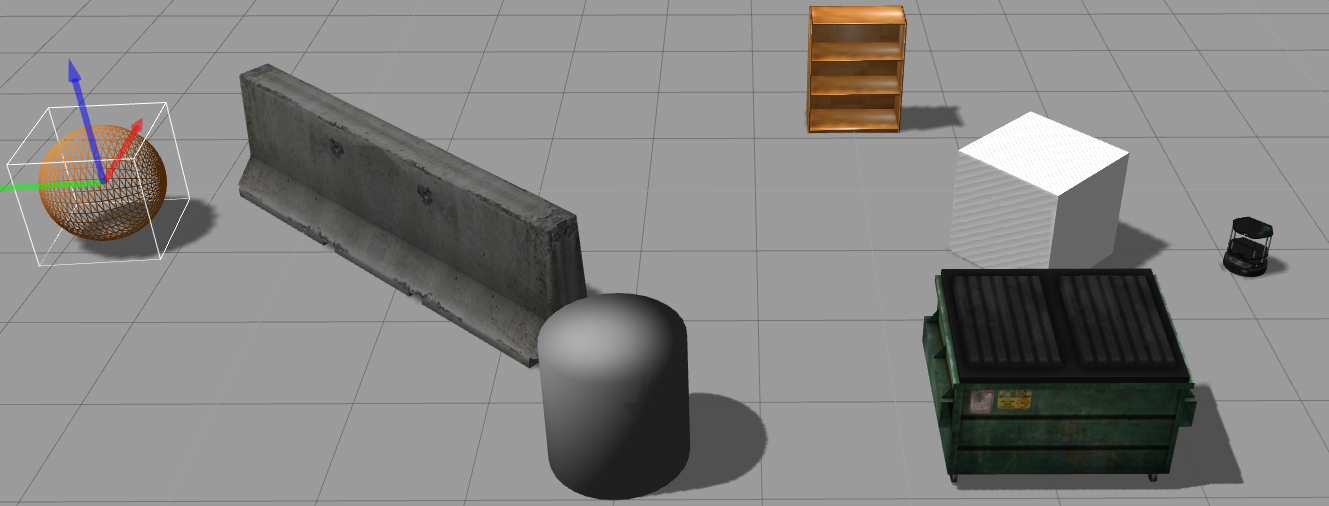
\includegraphics[width=0.49\textwidth]{scenario_3}
\caption{Dense obstacle path-planning scenario}
\end{figure}

\begin{figure}
\label{figure16} 
\centering 
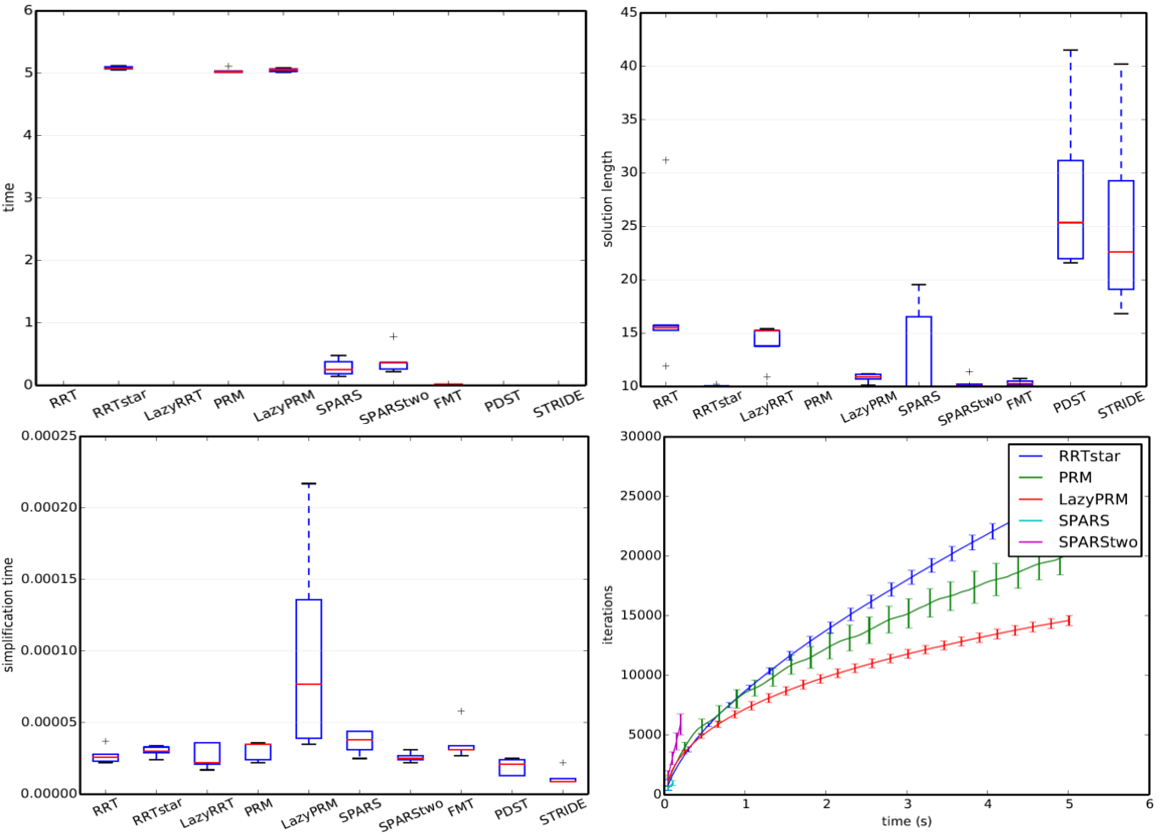
\includegraphics[width=0.49\textwidth]{s3_outcomes}
\caption{Dense obstacle scenario outcomes}
\end{figure}

The important graphs of algorithms during this run are tiled in figure 16. As before, all planners were able to find exact solutions to the planning problem. The planners in order 
from minimum to maximum amount of time were the following: PDST, STRIDE, FMT*, SPARS, SPARS2, PRM, LazyPRM, and RRT*. In terms of iterations, the order from least to greatest was 
the following: SPARS, SPARS2, LazyPRM, PRM, and RRT*. The SPARS planner took approximately 2,500 iterations to converge on average. The SPARS2 planner again took about 7,000 more iterations to converge than the SPARS planner at 9,500 iterations on average. 

The solution length statistics for this scenario differed from the previous two scenarios. It turns out that the only planners that produced nearly the shortest paths were The
SPARS2, FMT*, LazyPRM and SPARS planners. The other planners either converged to a larger local minimum or had a high amount of variance in solution length. The amount of time 
taken by the path simplification algorithm was not as consistent as previous scenarios this time. The total planning times in order from least to greatest are: STRIDE,
PDST, LazyRRT, RRT, SPARS2, RRT*, PRM, FMT, SPARS, and lastly, the LazyPRM.

In terms of time, the quickest planners were again the STRIDE, PDST, FMT*, SPARS, and SPARS2 planners. These all took less than 1 second to solve as usual.
In terms of solution length, the planners with the shortest solutions were the SPARS2, FMT* and LazyPRM planners. The other planners besides RRT had high amounts of variation in 
output. In terms of performance efficiency, the planners that were best off were the SPARS, SPARS2, STRIDE and PDST planner. In terms of solution smoothness, the best algorithms
were the PDST, LazyRRT, RRT, STRIDE, and LazyPRM planners, in ascending order. Lastly, in terms of minimal memory consumption, the top 
contenders were the RRT* and LazyRRT algorithms, due to their single query planning behaviour. The next runner up was the PRM algorithm, which had a high variance in measurement. 
These algorithms consumed less memory than all the other algorithms.

Given these outcomes, we can make a determination that either the SPARS2 or STRIDE algorithms would be the best planning algorithm for an environment with a dense obstacle 
distribution. The next runner up would be the PDST algorithm, but it produces solutions that are unnecessarily long without post-processing, which defeats the purpose of
having a well-rounded and efficient algorithm. 

\section{Benchmark Comparisons} \label{Benchmark Comparisons}
Given the several categories analysed throughout each benchmark scenario based on obstacle presence, some comparisons can be made across the board to determine the best planner
for all categories overall.

\subsection{Time Comparisons} \label{Time Comparisons}
The algorithms benchmarked in this paper all vary in runtime based on which scenario is in focus. There were some noticeable trends in the time taken to construct an accurate
solution to each posed path planning problem with the turtlebot. The SPARS, SPARS2, FMT*, STRIDE, and PDST methods stood out for their minimal construction and planning time.
These algorithms and the RRT family took minimal time to simplify, however, the LazyPRM solutions always took the most time to simplify due to their highly segmented nature.

\subsection{Length Comparisons} \label{Length Comparisons}
All solutions from certain planners were consistently in the top few for having the shortest solution path. Those certain planners were the SPARS and SPARS2 planners, not 
surprisingly at this point. The path lengths are almost always optimal with the SPARS2 planner, which sets the new bar for consistency in mobile robot path planning.

\subsection{Efficiency Comparisons} \label{Efficiency Comparisons}
The efficiency was surprisingly good for the RRT and PRM methods. The lazy collision checking versions of RRT and PRM proved to be much more efficient than their counterparts.
As in figure 17, a sample of the regular vs. lazy PRM node counts shows the lazy PRM develops many less nodes than other counterparts as expected given additions described in
\cite{lazy_prm}. However, despite the strong efficiency of the RRT and PRM, the SPARS planners again beat them, matched with competition from STRIDE and FMT*, SPARS2 always
selectively adds additional configurations to its graph with near-optimality performance only if they improve the path quality relative to paths on a dense graph. The only
downside to the SPARS2 method are its memory usage, but with the hardware in computers of today, memory consumption is a small issue compared to overall real-time performance.

\section{Results} \label{Results}

All in all, the benchmarks revealed neck in neck competition for the fastest, shortest, and smoothest solutions. As the goal being the ability to determine the best modern day
planner, there was only one real winner across the board -- the SPARS2 planner. This planner outperformed all other planners including its bigger brother the SPARS planner. 
As discussed in \cite{spars_two}, the planner was a modified version of the SPARS planner with enhancements for converging to a proper solution quickly over a certain amount of
time by not adding more nodes to the graph unless completely worthwhile as evaluated by a specific spanner property. This addition improves memory requirements and results
in the generation of smaller graphs shorter solutions than planners such as the LazyPRM, STRIDE, FMT*, PDST, and the earlier SPARS, in the long run.

\section{Conclusion} \label{Conclusion}

In conclusion, the SPARS2 planner is the suggested planner for use in future modern motion planning applications based on its strong place in the benchmark comparison.
Perhaps more work could be pursued in the future to implement this planner as the default in up and coming robotics in need of quick, accurate and efficient planning.

\printbibliography
\end{document}